In order to motivate the need for the APEX approach, we first outline the architecture of a typical ADAS/AV control system. 
It is \emph{not} necessary that a vehicle use this \emph{particular architecture} in order to be verified under APEX, but it motivates the key issues involved in obtaining a proof of safety. In the three-layer architecture paradigm \cite{Gat98} which we demonstrate, the planning and control of the vehicle is hierarchical in nature. Each successive layer performs a task over a shorter time horizon. Fig. \ref{fig:tla_new} details this approach to AV architecture.

\begin{figure}[h]
	\centering
	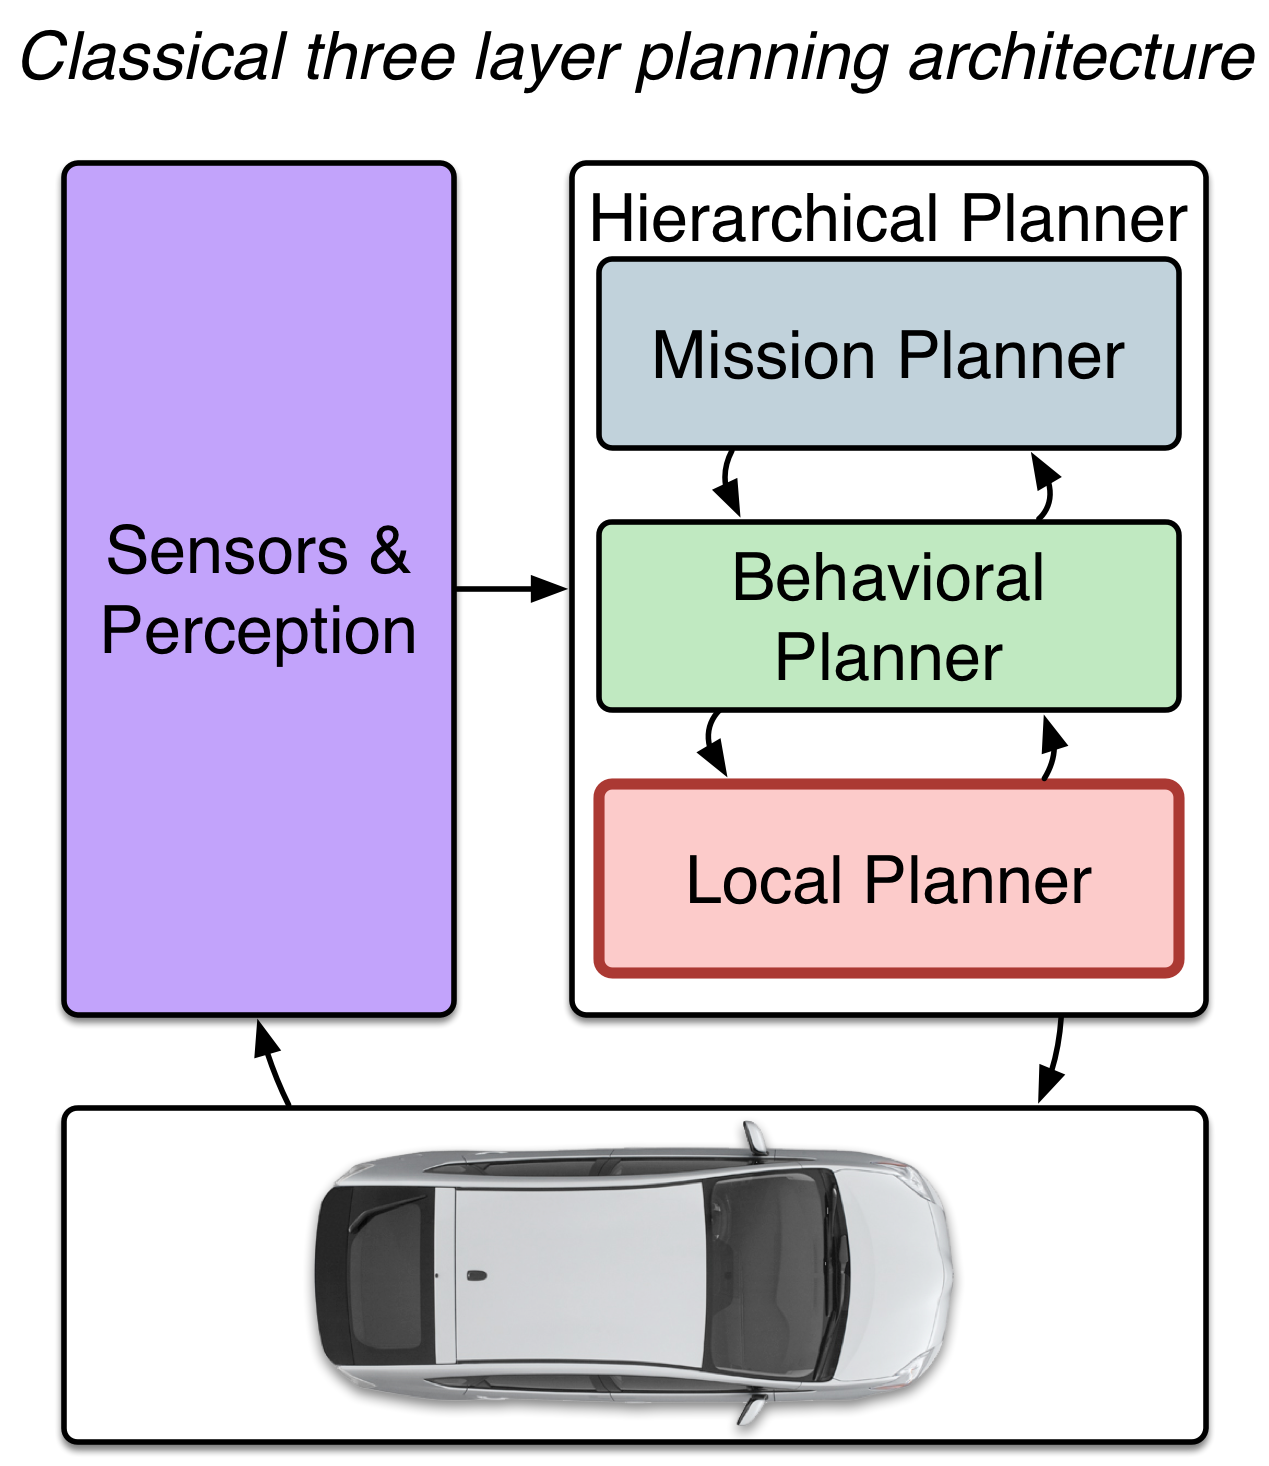
\includegraphics[scale=.3]{figures/tla_new.png}
	\caption{The three layer architecture presented by Gat is widely accepted as a standard means of implementing planning and control for an autonomous vehicle.}
	\label{fig:tla_new}
\end{figure}

At the top level a mission planner is given a mobility goal. Such a goal is typically expressed as a (location, destination) pair. Given this pair the mission planner finds an optimal (or feasible) route through the road network. 

In the next layer, the behavioral planner makes local decisions about how to navigate the road network. For example, if the mission planner informs the behavioral planner that at the next intersection it will need to turn left, the behavioral planner will use a set of rules to determine that the ego vehicle must be in the left lane.
It then provides a sequence of waypoints, or intermediary destinations, to the lower-level local planner. 

Finally, the local planner, or \emph{trajectory planner}, produces a trajectory that connects the vehicle's current pose to the target pose at the next waypoint. 
Here `pose' refers to the combined position, heading and velocity of the vehicle.
Specifically, given a goal pose relative to the vehicle's current pose, the local planner computes a set of candidate smooth trajectories that can lead to the goal pose or near it, then selects a single trajectory and sends it to the vehicle. 
The vehicle itself includes a PID controller (or some other controller) that makes it track the selected trajectory.